%!TEX root = thesis.tex

\renewcommand{\TheTitle}{Influence of Multiple Firebrands on the Ignition of Fuel Beds}
\renewcommand{\TheAuthors}{Derek Bean, David L. Blunck \\ \\ My contributions to this work included the design of the experiments, fabrication of the experimental apparatus, collecting data, data analysis, modelling efforts, and preparation of the manuscript.}

\renewcommand{\TheAddress}{
\textbf{Status: In Preparation}\\
Target Journals: Fire Safety Science, Fire Safety Journal, or Fire Technology
}

\PaperHeader{\TheTitle}{\TheAuthors}{\TheAddress}

\chapter{\TheTitle}
\label{part:manuscript4}

\section{Abstract}
    some text
\section{Introduction}
    The increase of both wildfire severity and the number of homes on the Wildland Urban Interface (WUI) has increased the occurrence of home loss due to wildfires since the turn of the century~\cite{Manzello2013}. Ignition of fuels by firebrands that in turn leads to the loss of a structure is a primary source of home loss~\cite{Koo2010a, Syphard2019, Roberts2021}, and in some fires has been the source of 2/3 of structure ignitions~\cite{Maranghides2013NISTIgnitions}. Thus, it is important to understand the ignition of fuel beds by firebrands in order to mitigate the risk of ignition~\cite{Manzello2014}. Ideally, the understanding of the ignition process would result in a predictive model that would enable homeowners, firefighters, and other risk management personnel to determine location specific strategies for preventing ignition before and during a fire. Unfortunately, such a model does not currently exist due to critical shortfalls in the current knowledge of fuel bed ignition. For example, if a burning twig or cone landed on needles accumulated in a gutter of a home there is no model that can quantitatively predict whether or not ignition occurs and therefore the risk of that structure being lost to ignition from the ember cannot be determined. The consequences of not being able to determine loss risk for structures are numerous. For example, in WUI fires firefighting resources are often used to harden homes against firebrand ignition but without an accurate prediction of risk each home must be treated equally which in turn spends fixed resources on homes that don't need assistance at the detriment to those at highest risk. 
    
    Processes that influence ignition begin within the fire when an firebrand (e.g., branch, bark, cone etc) is ignited and lofted into the air by wind. The combusting firebrand is then transported to and lands on a fuel bed near or on a structure. Energy is then transferred to the fuel bed and if the energy is sufficient the fuel bed will undergo pyrolysis and produce flammable gases which may then ignite and begin flaming. These flames may then spread and destroy the structure. Each of these processes, firebrand generation, transport, and ignition, require additional research before a predictive model is possible. This work focuses on the processes that occur during ignition of the fuel bed.
    
    An additional risk factor for the ignition of structures is the accumulation of firebrands on fuel beds. The geometry of homes often promotes the accumulation of firebrands by creating recirculation zones which promote the deposition of firebrands. The accumulation of firebrands poses an increased risk of home ignition in multiple ways. First, since ignition is largely a stochastic process, the more firebrands that land on an area the larger the probability of ignition. Second, firebrands that accumulate close to one another creating piles may depart more energy onto a fuel bed than a single firebrand alone. In work conducted by Hakes et al.~\cite{Hakes2019a} an increase in firebrand pile mass increased the total energy imparted to an instrumented surface. The increase in energy release was attained by a longer duration of energy release as the pile mass increased.
    
    The accumulation of firebrands near structures also requires the presence of wind which has also been shown to influence ignition. The presence of wind has been shown to decrease the threshold of ignition. In work conducted by Suzuki and Manzello~\cite{Suzuki2020a} when wind was increased from 6\si{\meter\per\second} to 8\si{\meter\per\second} the number of firebrands required for ignition of the wood much fuel bed decreased. Similar observations of wind lowering the ignition threshold have been observed in multiple studies with single firebrands. Wang et al.~\cite{Wang2017} reported decreases in ignition times as wind speed increased for hot metal particles dropped on pine needle fuel beds. Ellis reported that the addition of wind increased the threshold of fuel moisture content where ignition was observed for natural firebrands  deposited on eucalypt forest litter. The trends observed by Ellis agreed with those observed by Ganteaume et al.~\cite{Ganteaume2009} and Pulcinski and Anderson~\cite{Plucinski2008} where the addition of wind increased ignition probability. From these studies an increase of wind increases the danger of fuel bed ignition near homes but the mechanism(s) that cause the increased ignition probability are unclear. 
    
    For single firebrands it has been postulated that the primary enhancement of wind is due to increased oxygen to the firebrand and fuel bed. From these works it was unclear if the ignition enhancement was due to increased heat release from the firebrand, increased mixing and oxygen in the pyrolyzates, or some combination of both. Results from the work outlined in Chapter~\ref{part:manuscript2} show that in the presence of an ignition source where the heat release is not influenced by wind an increase of wind increases the ignition probability. The increase in ignition probability was attributed to the accumulation of pyrolysis products near the energy source (cartridge heater) suggesting that fluid flow near the firebrand is a significant controlling parameter for ignition. 
    
    The addition of multiple firebrands in close proximity adds additional layers of complexity with respect to both heat release and fluid dynamics.  Hakes et al.~\cite{Hakes2019a} identified re-radiation and reheating as key processes that differentiate single firebrands from multiple firebrands and have significant influence on energy deposited to the fuel bed.  The presence of multiple firebrands may also create disturbances in the fluid flow around the firebrands that influence recirculation zones and alter the ignition propensity. What is unclear from these conclusions is the magnitude of the effect that re-radiation and flow disturbances have on ignition. Understanding the magnitude of these processes on the probability of ignition is imperative to creating accurate ignition models. 
    
    With this background and motivation, the objective of this study is to quantify the influence of multiple firebrands on the ignition propensity of a fuel bed. It is anticipated that the results of this work will help further the understanding of the difference in ignition propensity between a single firebrand and multiple firebrands that may interact through fluid and thermal processes. A more complete understanding of these processes will enable an increased accuracy of ignition models and better protection of structures in the WUI.
    
    
\section{Methodology}
    The probability of flaming ignition for fuel beds consisting of Douglas-fir particles was measured for eight configurations of two firebrands in a wind tunnel. The wind tunnel was operated at either 0.5 \si{\meter\per\second} or 5.8 \si{\meter\per\second} for each test series. The wind speed was measured with a TSI-IFA300 hot wire probe. Figure~\ref{fig:multiHeaterApparatus} shows a representation of the wind tunnel, fuel bed, and the automated lowering device. Table~\ref{tab:multiHeaterConfig} shows the test matrix for each series of tests. For all of the tests the heaters were oriented perpendicular to the flow and the downstream heater was heated. For tests where both heaters were heated the temperatures of both heaters were maintained at the same temperature. 
    
    The combinations of heater spacing and hot or ambient upstream heater were chosen to represent different levels of fluid and thermal interactions between the heaters and the fuel bed. The heater spacing of five diameters was chosen such that minimal interaction between the heaters occurs as previous CFD calculations indicate that the recirculation zone of the upstream heater is approximately five diameters when the heater is in a wind of 5.8 \si{\meter\per\second} and an orientation perpendicular to the flow. Preliminary thermal calculations also indicated that the pyrolysis fronts created by each heater are unlikely to interact within previously observed times to ignition. The heater spacing of one diameter was chosen for a high level of interaction between both the fluid disturbances and thermal fronts of each firebrand. The one diameter spacing places the downstream heater inside the recirculation zone of the upstream heater under wind and the preliminary heat transfer calculations indicated that the thermal fronts of each heater will merge before the anticipated time to ignition. The chosen heater orientations also represent potential scenarios that may be encountered in a wildfire. The configuration with two heaters both heated is representative of a multi firebrand attack where the one diameter spacing approximates a firebrand pile and the five diameter spacing approximates two firebrands falling in close proximity but not within each others region of influence. The configuration with only the downstream heater heated is representative of an firebrand falling near an object (e.g., twig, rock, or cone) that disturbs the flow and may act as a heat sink for the energy deposited to the firebrand with the one and five diameter spacing representing an firebrand falling both within and outside of the region of influence of the firebrand. The configuration where the upstream heater is not heated and five diameters is also considered a control for comparison to previous single heater ignition results.
    
            \rowcolors{2}{gray!25}{white}
        \begin{table}[hpbt]
            \normalsize
            \caption{Test matrix}
            \centering
            \begin{tabular}{ccccr}
                \rowcolor{gray!50}
               Test Series & Heater Spacing & Upstream Heater & U\textsubscript{bulk} (\si{\meter\per\second})\\
                \hline
                1   & 1 & Ambient & 0.5 \\
                2   & 1 & Ambient & 5.8 \\
                3   & 1 & Hot     & 0.5 \\
                4   & 1 & Hot     & 5.8 \\
                5   & 5 & Ambient & 0.5 \\
                6   & 5 & Ambient & 5.8 \\
                7   & 5 & Hot     & 0.5 \\
                8   & 5 & Hot     & 5.8 \\
            \end{tabular}
            \label{tab:multiHeaterConfig}
        \end{table}
    
    The cartridge heaters used had diameters of 6.4\si{\milli\meter} and lengths of 51\si{\milli\meter}. The heater sizes were chosen to represent large firebrands with a high potential to ignite a fuel bed in a wildfire~\cite{Manzello2007}. The heater temperatures were controlled using a PID temperature controller implemented in LabVIEW. Heater temperatures ranged from 250\si{\celsius} to 750\si{\celsius}. Heater temperatures were measured using a type-K thermocouple attached to the center of each heater opposite the fuel bed.
    Controlling the temperature of the heater provides an advantage over natural burning or smoldering firebrands and pre-heated particles by removing the temperature variability of the heat source and enabling real time data logging of the heat source temperature. Controlling the temperature of the firebrand also removes some complexity of calculating the energy imparted to the fuel bed. The heater was lowered onto the fuel bed with an automated lowering device. The lowering device included a load cell and a PID controller to maintain a force equivalent to a two 10\si{\gram} firebrands throughout the experiment. To minimize flow disruptions due to apparatus the heaters were each attached to two 4-40 threaded rods that extended approximately 100\si{\milli\meter} below the load cell. 
    
         \begin{figure}[hbpt]
            \centering
            \resizebox{0.5\columnwidth}{!}{%
                \begin{tikzpicture}
                    \filldraw[pattern=north west lines, pattern color=brown, thick] (2.84, 0)  rectangle (4.34, -.75) node[pos=0.5,rectangle,fill=white] {\scriptsize Fuel Bed};
                    \fill [draw=white,  inner color=red, outer color=white ] (3.43, 0.01) circle (0.15);
                    \fill [draw=white,  inner color=red, outer color=white ] (3.74, 0.01) circle (0.15);
                    \filldraw[draw=black,fill=white, thick] (0, 0)      rectangle (6, 3);
                    \fill[fill=black!50] (3.41, 0) rectangle (3.44, 1.40);
                    \fill[fill=black!50] (3.72, 0) rectangle (3.75, 1.40);
                    \fill[fill=black] (3.55, 1.52) rectangle (4.23, 1.57);
                    \fill[fill=black] (3.55, 1.45) rectangle (3.60, 1.52);
                    \filldraw[draw=black, fill=black!50] (3.3, 1.40) rectangle (3.86, 1.45);
                    \filldraw[draw=black, fill=black!50] (4.09, 1.57) rectangle (4.22, 3);
                   
                    
                    \draw [<-] (3.5, 1.55) -- (3, 1.55) node[left] {\scriptsize Load Cell};
                    \draw [<-] (3.75, 2.5) -- (3, 2.5) node[left] {\scriptsize Lowering Arm};
                    \draw[->]         (0.1, 0.6) -- (0.75, 0.6);
                    \draw[->]         (0.1, 1.2) -- (0.75, 1.2);
                    \node[right] at (-0.75, 1.5) {\scriptsize Inlet};
                    \draw[->]         (0.1, 1.8) -- (0.75, 1.8);
                    \draw[->]         (0.1, 2.4) -- (0.75, 2.4);
                    \draw[draw=black, dashed] (2.84 , 0) rectangle (4.34, 0.7);
                    \draw[->]         (4.3, 1) -- (4.0, 0.34);
                    \node[right, align=left] at (4.3, 1) {\scriptsize Computational\\ \scriptsize Domain};
                    \fill[draw=red, fill=red] (3.43, 0.01) circle (0.0635);
                    \fill[draw=red, fill=red] (3.74, 0.01) circle (0.0635);
                    \draw [<-] (3.4, 0.1) -- (2.85, 0.5) node[left] {\scriptsize Heaters};
                \end{tikzpicture}
                }
            \caption{Diagram of the experimental wind tunnel apparatus. Air flows through the wind tunnel from left to right. The dashed region represents the domain subset used for computational efforts.}
            \label{fig:multiHeaterApparatus}
        \end{figure}
    
    The fuel bed material was processed from kiln dried Douglas-fir lumber. The lumber was first planed to generate shavings. The wood shavings were then granulated and screened such that the particles passed through a 2.3\si{\milli\meter} screen but not through a 1.3\si{\milli\meter} screen. The particles were then dried in an oven at 103\si{\celsius} to remove any remaining moisture content. During tests, the fuel was placed in a 140\si{\milli\meter} diameter glass container with a depth of 70\si{\milli\meter} and then inserted into the wind tunnel. The average density of the fuel beds was XX.X\si{\kilo\gram\per\cubic\meter}.
    
    A simplified model was implemented to obtain further insight into the fluid mechanics and heat transfer processes that influence the trends observed in the experimental efforts. The model was implemented in three parts. First, a thermal model of the fuel bed was used to estimate the mass of the fuel bed above the pyrolysis temperature and the average temperature. Second, the mass of the fuel bed material converted from solid fuel to gaseous pyrolysis products was estimated. In the third and final step the fluid flow and heat transfer between the heaters, air, and released pyrolyzates was modeled. The modelling efforts were conducted for a 10\si{\second} interval to ensure proper characterization of the flow field and maintain an accurate representation of the fuel bed. As mass is lost from the fuel bed due to pyrolysis the contact area between the heater and the fuel bed changes as does the surface shape of the fuel bed. It was observed during experiments that the contact between the heat and the fuel bed and the shape of the fuel bed itself began to deviate significantly from the model domain at approximately 10\si{\second}. Considerations of changes in contact area and changing geometry due to pyrolysis is out of the scope of this work. Nonetheless, the treatment of each configuration equally and within the limited time frame is still anticipated to produce insight into the influence of the thermal and fluid processes on ignition. 
    
    The thermal model of the fuel bed was conducted using OpenFOAM~\cite{Foundation2020}. Figure~\ref{fig:multiHeaterThermal} shows the computational domain of the fuel bed. The thermal diffusivity of the fuel bed materials was estimated using correlations from literature for the thermal conductivity~\cite{bergman2011fundamentals} and published values of specific heat~\cite{Parker1986}. Equation~\ref{eqn:estk4} shows the the correlation for effective thermal conductivity where $\epsilon$, as defined in Equation~\ref{eqn:epsilon4}, is the proportion of the fuel bed that is air. The bulk density of the fuel bed material ($\rho_{bed}$) and the solid wood ($\rho_{solid}$) were obtained from experimental samples. 
        \begin{equation}
            k_{eff} = \frac{1}{2} \left(\frac{1}{\left( 1 - \epsilon \right)/k_{solid} + \epsilon/k_{air}} +  \epsilon k_{air} + \left(1-\epsilon \right) k_{solid} \right)
            \label{eqn:estk4}
        \end{equation}
        \begin{equation}
            \epsilon = 1- \frac{\rho_{solid}}{\rho_{bed}}
            \label{eqn:epsilon4}
        \end{equation}
    The interface between the fuel bed and air and the radial edge of the domain were treated as insulated. The centerline was treated as a symmetric boundary condition. The insulated radial edge and symmetric boundary condition are consistent with boundary conditions in the actual experiment since the 25\si{\milli\meter} distance ensures no temperature change during 10\si{\second} of heating modeled and the heater temperature has been observed to be circumferentially consistent with infrared imaging. The insulated interface with the air does not account for radiation and convective heat losses from the surface of the fuel bed as it is heated. However, the magnitude of the heat losses from the fuel bed is estimated to be significantly smaller in magnitude than the heat transfer from the heater. Reactions, mass loss due to pyrolysis, and changes in contact area due to changing fuel bed geometry are not considered in the temperature analysis. While the aforementioned assumptions and limitations reduce the accuracy of the model in comparison to the experimental conditions, the temperature distributions still provide insights into differences in the mass of the fuel bed material that undergoes pyrolysis and provides insight to better interpret the experimental results. 
    \begin{figure}
        \centering
        \resizebox{0.375\textwidth}{!}{%
          \begin{tikzpicture}
            \node at (0,0) (origin) {};
            %\draw (origin) rectangle (topright);
            \fill[pattern=north west lines, pattern color= brown, draw=black] (3.18mm, 0) -- (25mm, 0) arc (0:-90:25mm) -- (0, -3.18mm) arc (270:0:3.18mm ) -- cycle ;

            \node (text) at (12mm, -12mm) {Fuel Bed};
            \fill [draw = white,  inner color=red, outer color=white ] (0mm, 0mm) circle (10mm);
            \fill [draw=white, fill=white] (0,0) -- (10mm, 0) arc(0:270:10mm) -- (0,0);
            \filldraw [fill=white, draw=red, thick] (0, 0) circle (3.18mm);

            \fill[pattern=north east lines, pattern color=black!90] (-2mm,-3.18mm) rectangle (0mm,-27mm) node[rotate=-90, pos=0.5] {};
            %\fill[pattern=north east lines, pattern color=black!90] (0mm,-2mm) rectangle (27mm,0mm) node[rotate=-90, pos=0.5] {};
           \fill[pattern=crosshatch] (25mm, 0) -- (27mm, 0) arc (0:-90:27mm) -- (0, -25mm) arc(-90:0:25mm) ;
            \draw[-stealth,decorate,decoration={snake,amplitude=1pt,pre length=0pt,post length=2pt}] (3.5mm, -6mm) -- ++(1mm, 9mm);
            \draw[-stealth,decorate,decoration={snake,amplitude=1pt,pre length=0pt,post length=2pt}] (6mm, -5mm) -- ++(1mm, 7mm);
            \draw [|-|] (-5mm, 0mm) -- (-5mm, -25mm) node[pos=0.5, left] {25mm} ;
             \draw[thick, dashed] (3.18mm, 0) -- (10mm, 0);
            \draw (0mm, -3.18mm) -- (0mm, -10mm);
            \node[draw, rectangle, fill=white, draw=white] (p) at (8mm, 10mm) {Pyrolysis Gases};
	        \draw[->, thick] (p.south) -- (6mm, 2mm);
	        \node[draw, rectangle, fill=white, draw=white, anchor=west] (p) at (12mm, 4mm) {T=220\si{\celsius}};
	        \draw[->, thick] (p.west) -- (10mm, 1mm);
          \end{tikzpicture}
          }
        \caption{Diagram of the computational domain where black lines indicate domain boundaries, and red lines are boundaries defined by the heater. The arrows denote flow of pyrolysis products from the fuel bed into the air above the fuel bed.}
        \label{fig:multiHeaterThermal}
    \end{figure}
    
    The velocity of pyrolyzates entering the fluid domain from the fuel bed was determined in a two step process. First the mass of material in the fuel bed undergoing pyrolysis was estimated. All material over a temperature of 220\si{\celsius} was considered to undergo pyrolysis. This temperature was chosen as 220\si{\celsius} corresponds to the minimum temperature for the pyrolysis of hemicellulose and is considered the onset of pyrolysis~\cite{Yang2007a}. The amount of mass estimated to depart the fuel bed was determined to be the proportion of fuel bed material that converted to gas phase products when reacted at the average temperature of the material above the pyrolysis threshold from the thermal model. Reactions were conducted using the BioPOx mechanism~\cite{Dhahak2019} and mass was assumed to depart the fuel bed if it existed in the gas phase. Species were considered to be gas phase if they were present in the Bio1412 mechanism~\cite{Ranzi2001, Ranzi2008}, since the Bio1412 mechanism considers the gas phase reaction of pyrolysis products. The reaction calculations were conducted in Cantera~\cite{Goodwin2020}. The Cantera calculations were 0D which necessitated using the average temperatures of the fuel bed for the pyrolysis calculations rather than spatially resolved temperatures. Mass flux of the gases exiting the fuel bed was determined by averaging the total mass of gaseous pyrolysis products produced over the 10\si{\second} interval. The exit velocity was then determined as the mass flux through the distance between the the heater edge and the pyrolysis threshold as shown by the dotted line in Figure~\ref{fig:multiHeaterThermal}. The calculated velocity and injection area was then used as an input for calculations conducted in the flow field. 
    
    A 2D RANS model of the flow above the fuel bed and around the heaters was implemented in OpenFOAM. The area of the computational domain with respect to the experimental apparatus is shown as the dashed line in Figure~\ref{fig:multiHeaterApparatus}. The 2D slice of the domain modeled was considered to pass through the center of the heaters and corresponds to the location of the highest temperature of the heater which also typically coincides with the ignition location. Turbulence parameters were determined from measurements taken of the experimental apparatus with a TSI IFA-300 hot wire anemometer. The k-$\epsilon$ turbulence model was used with values of 1.4$\cdot$10\textsuperscript{-4}\si{\square\meter\per\square\second} and 9.5$\cdot$10\textsuperscript{-6}\si{\square\meter\per\cubic\second} for k and $\epsilon$ respectively. Calculations were conducted for 10\si{\second} and were then averaged to observed differences in temperature and velocity characteristics between the different configurations. 
    
    
\section{Results and Discussion}
    The flaming ignition or non-ignition result of each test is shown in Figure~\ref{fig:multi_heater_hot_vs_ambient}. The markers show the result of each test and the the curves show the logistic regression for each of the heater configurations as defined in Table~\ref{tab:multiHeaterConfig}. The shaded regions around the curves represent the 95\% confidence intervals of each regression. The top plot in Figure~\ref{fig:multi_heater_hot_vs_ambient} shows configurations where the downstream heater is actively heated and the upstream heater is at ambient conditions. The bottom plot in Figure~\ref{fig:multi_heater_hot_vs_ambient} shows results for configurations where both heaters are actively heated to the same temperature.
        \begin{figure}[hpbt]
            \centering
            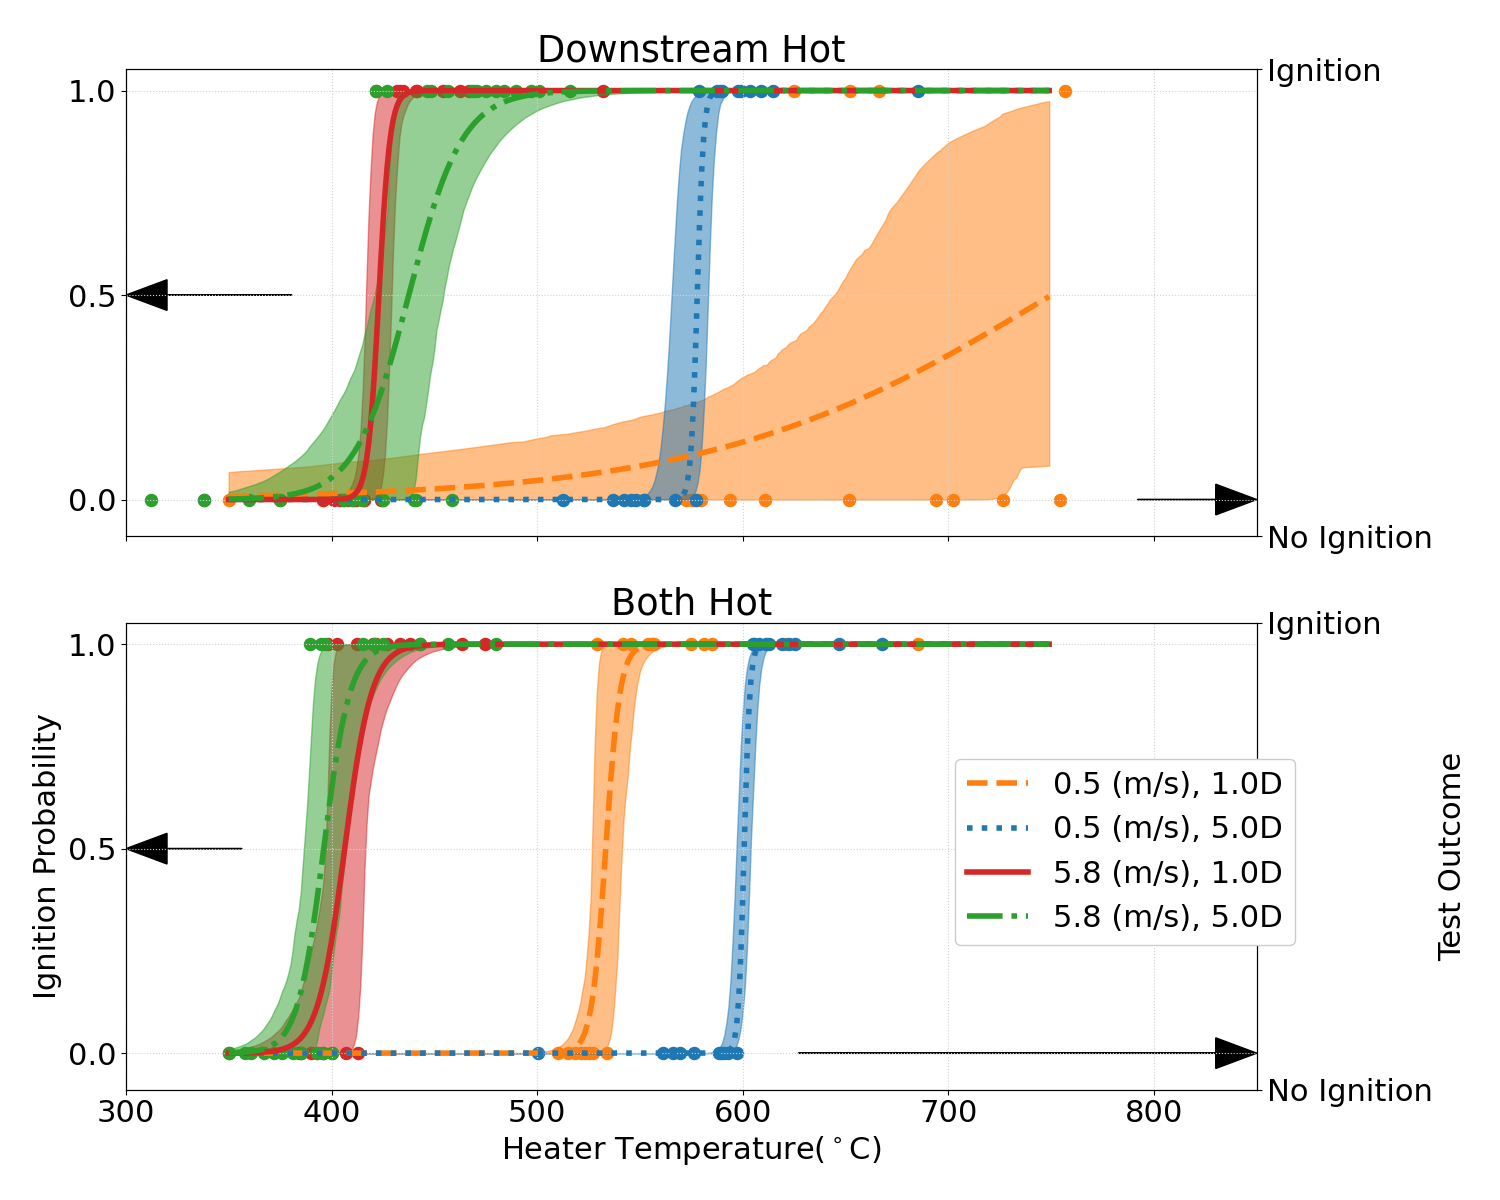
\includegraphics[width=0.75\columnwidth]{Figures/multi_heater_plot.png}
            \caption{Ignition or no ignition outcomes of tests with different heater configurations. The circular markers indicate outcomes of individual tests and the curves represent logistic regressions of each test series. The shaded region shows the 95\% confidence interval for each regression.}
            \label{fig:multi_heater_hot_vs_ambient}
        \end{figure}
    Table~\ref{tab:multiFiftyTemp} shows the heater temperatures estimated to result in a 50\% ignition probability from the logistic regressions shown in Figure~\ref{fig:multi_heater_hot_vs_ambient} as well  Temperature values for the corresponding wind speed and orientation from the single heater study in Chapter~\ref{part:manuscript2} are shown in the column titled "Single" for comparison. 
        \rowcolors{2}{gray!25}{white}
        \begin{table}[hpbt]
            \normalsize
            \caption{Heater temperature required to achieve 50\% ignition probability for the configurations tested with 95\% confidence intervals shown in parentheses. The column "Unheated" refers to cases where the upstream heater was not temperature controlled and "Heated" refers to cases where both upstream and downstream heaters were maintained at the setpoint temperature. The single heater column shows the values from the study in Chapter~\ref{part:manuscript2} for a single heater.}
            \centering
            \begin{tabular}{ccrrr}
                \rowcolor{gray!50}
               U\textsubscript{bulk} (\si{\meter\per\second}) & Spacing (D) & Unheated (\si{\celsius})& Heated (\si{\celsius}) & Single (\si{\celsius})\\
                \hline
                0.5  & 1 & 750 (644, 850) & 533 (527, 541) & 571\\
                0.5  & 5 & 578 (565, 583) & 601 (597, 604) & 571\\
                5.8  & 1 & 423 (417, 429) & 406 (397, 416) & 399\\
                5.8  & 5 & 438 (421, 454) & 396 (387, 407) & 399
            \end{tabular}
            \label{tab:multiFiftyTemp}
        \end{table}
        
    Considering first the cases where both heaters are actively heated (Figure~\ref{fig:multi_heater_hot_vs_ambient} bottom panel and Table~\ref{tab:multiFiftyTemp} "Heated" column) there are three observations of note. First, in both the one and five heater diameter spacing cases an increase in wind from \textit{0.5\si{\meter\per\second}} to \textit{5.8\si{\meter\per\second}} resulted in a lower temperature threshold for ignition. The 50\% ignition threshold decreased 24\% (127\si{\celsius}) for the one diameter spacing and 34\% (205\si{\celsius}) for the five diameter spacing configuration. These results are similar to the 35\% decrease in the ignition threshold for the single heater results presented in Chapter~\ref{part:manuscript2}. The reduction in ignition temperature is attributed to an increased residence time of pyrolyzates near the heater in recirculation zones enabling ignition at lower temperatures. The second observation for the 0.5\si{\meter\per\second} wind speed tests is that decreasing the heater spacing from five heater diameters to one heater diameter resulted in an 11\% decrease in the temperature required for 50\% ignition probability. The shift in ignition probabilities is attributed to increased heat transfer between the closely spaced heaters. Anecdotally, the shift in ignition probability observed by moving the heaters closer together was accompanied by a shift in ignition mode. As the heater temperature was reduced below the 50\% ignition threshold for a single heater, ignition was observed only after the smoldering fronts between the heaters merged and ignition occurred in the plume of pyrolyzates that established between the heaters. The lower threshold for ignition when both heaters were heated and only one diameter apart is attributed to increased increased heat transfer to the pyrolyzates as they depart the fuel bed. It is not clear from these results what specific mechanism is the driving factor. Possibilities include increased temperature of pyrolyzates departing between the heaters due to to enhanced radiative and convective heat transfer, preheating of air as it flows over the upstream heater before mixing, increased mass flux of pyrolyzates from the fuel bed, or a combination of effects. In contrast to the differences in ignition at a wind speed of 0.5\si{\meter\per\second} the differences in ignition probability were not statistically significant at 5.8\si{\meter\per\second}. This suggests that the enhanced heat transfer between the cartridge heaters is not influential in windy conditions. Anecdotally, in cases under wind ignitions were to occur on the upstream side of the upstream cartridge heater suggesting that ignition is more favorable in the recirculation zones on the upstream side of the heater even with the addition of heat and pyrolysis.
   
    Now considering the cases where the only the downstream heater was actively heated there are three observations of note. First, similar to the dual heated and single heater results from Chapter~\ref{part:manuscript2} an increase of wind from an increase of wind from 0.5\si{\meter\per\second} to 5.8\si{\meter\per\second} significantly lowered the ignition threshold. Second, for cases with a wind speed of 5.8\si{\meter\per\second} changing the spacing between the heaters did not have a significant influence on the temperature required for ignition which aligns with the trends observed for the cases where both heaters were hot. Third, decreasing the spacing from five diameters to one diameter in low wind speed conditions increased the temperature required for ignition by greater than 30\% which is opposite trend observed for cases where both heaters were hot. This notable deviation from trends is attributed to the unheated heater acting as a heat sink requiring significantly more energy for ignition. 
    
    Further insight into the influence of heater configuration and wind speed on ignition is gained from the results of the computational efforts. Figure~\ref{fig:multiHeaterCFD} shows the averaged velocity streamlines and temperature distribution in the fluid flow around the heaters for each heater configuration. Air flows from left to right in Figure~\ref{fig:multiHeaterCFD}. The numbers inside the circular heater boundaries correspond to the assigned temperature of the heater during the calculation. The assigned surface temperatures correspond to the heater temperature anticipated to produce a 50\% probability of ignition for the wind speed and heater conditions. Heater boundaries with blue circles inside them correspond to cases where the heater was not heated and acted as an inert object. The arrows indicate the observed location of ignition, when observed. Ignition locations were not observed for every case, however, sufficient ignition locations were recorded to provide insight into controlling parameters.
        \begin{figure}
            \centering
            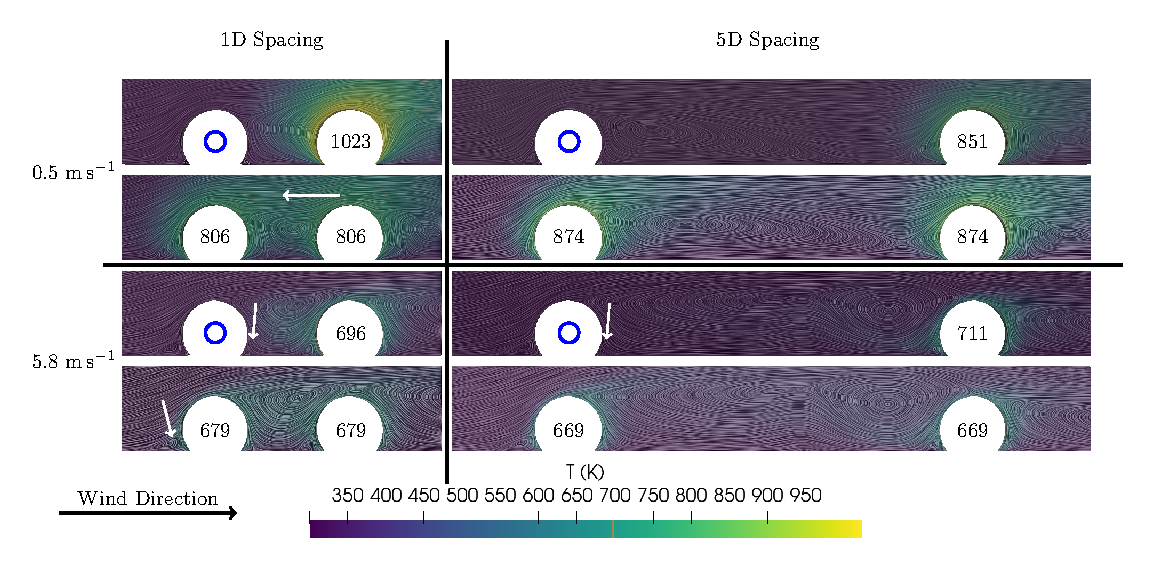
\includegraphics[width=\columnwidth]{Figures/quarter_circle.pdf}
            \caption{Time averaged velocity streamlines and temperature profiles for each configuration. The numbers inside of the heater boundaries identify surface temperature of the heater. Blue circles indicate that the heater was unheated and acting as an inert object. Arrows typical ignition locations.}
            \label{fig:multiHeaterCFD}
        \end{figure}
    
\section{Conclusions}
    Conclusions for this manuscript will go here. 